\begin{figure}[h]
\uwsinglespace
\begin{center}
\begin{minipage}{0.8\textwidth}
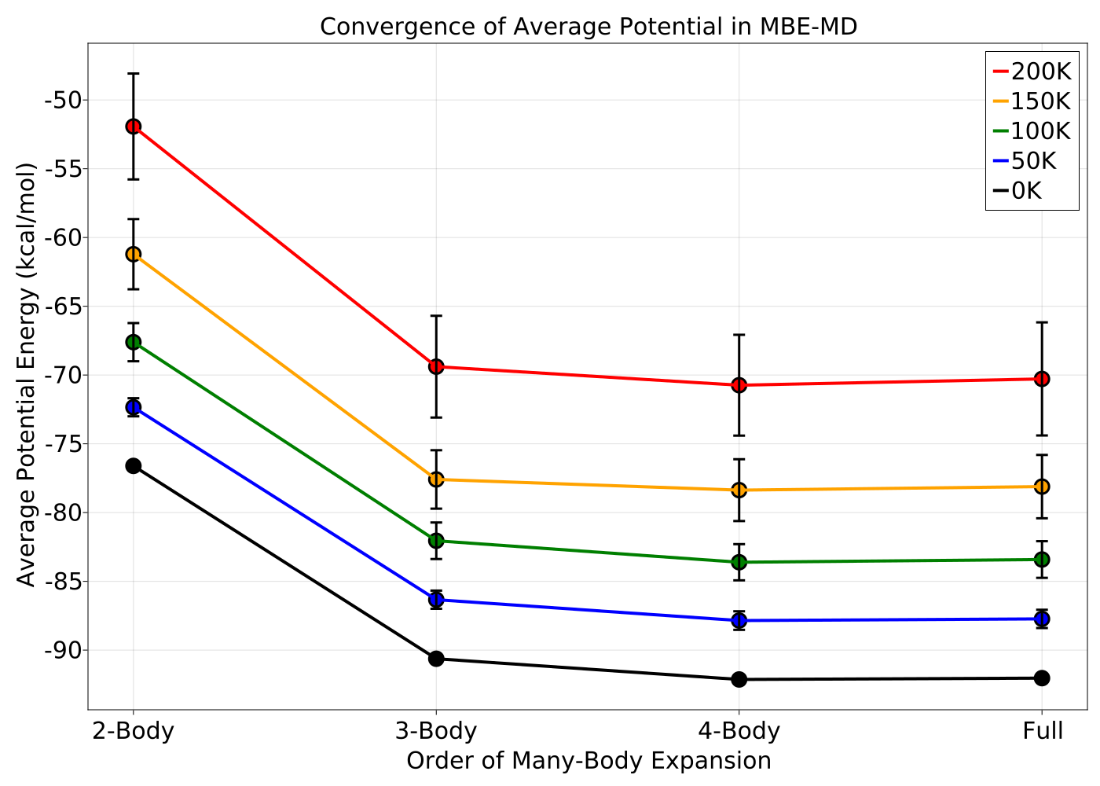
\includegraphics[width=\textwidth]{Figures/Chapter_4/ch4_figure_3.png}
\end{minipage}
\end{center}
\caption[Convergence of the average potential energy from MBE-MD at T=50K, 100K, 150K, and 200K when driven with a 2-, 3-, and 4-body representation of the potential. Error bars show the standard deviation of the average potential energy. Note that these do not represent uncertainties in the average energy, but the intrinsic fluctuations in potential energy due to thermal energy. The T=0K data correspond to an MBE from single point energies calculated on the minimum of the full PES.]{Convergence of the average potential energy from MBE-MD at T=50K, 100K, 150K, and 200K when driven with a 2-, 3-, and 4-body representation of the potential. Error bars show the standard deviation of the average potential energy. Note that these do not represent uncertainties in the average energy, but the intrinsic fluctuations in potential energy due to thermal energy. The T=0K data correspond to an MBE from single point energies calculated on the minimum of the full PES.}
\label{fig:MBE_MD_F3}
\end{figure}